\documentclass{article}

\usepackage[english]{babel}
\usepackage{amsmath}
\usepackage{amssymb}
\usepackage{float}
\usepackage{graphicx}
\usepackage{listings}
\usepackage{pdfpages}
\usepackage{tikz}
\usepackage{xcolor}
\usepackage{ulem}
\usepackage{subcaption}
\usepackage{geometry}
\usepackage{hyperref}
\usepackage{algorithm}
\usepackage{algpseudocode}
\usepackage{multirow}

\newcommand{\code}[1]{{\texttt{#1}}}

\usetikzlibrary{shapes.geometric,calc,shadows.blur,decorations.pathmorphing,fit,decorations.pathreplacing}
\bibliographystyle{unsrt}

\title{Example Manuscript}

\begin{document}

\section*{Introduction}

Although the manuscript should be considered as optional in a project like this, there are some advantages if done properly and in \LaTeX. Certain IDEs (e.g. Visual Studio Code) allow you to work on the manuscript (.tex file) and the code (.py file) in the same environment. This way, every change in the resulting figures will immediately be reflected in the manuscript. 

\section*{Mandelbrot Set}

The Mandelbrot set mentioned in the code in \code{'Code/MandelbrotCode\_(Commented)'} arises when you iterate the sequence 
\begin{equation}
    \label{eq:mandelbrot}
    z_{n+1} = z_n^2 + c
\end{equation}
for a complex number $c$. The set is defined as the set of all complex numbers $c \in \mathbb{C}$ for which the sequence $(z_n)_{n\in \mathcal{N}}$ does not diverge. The result can be approached numerically and is shown in Figure \ref{fig:mandelbrot}.

\begin{figure}
    \centering
    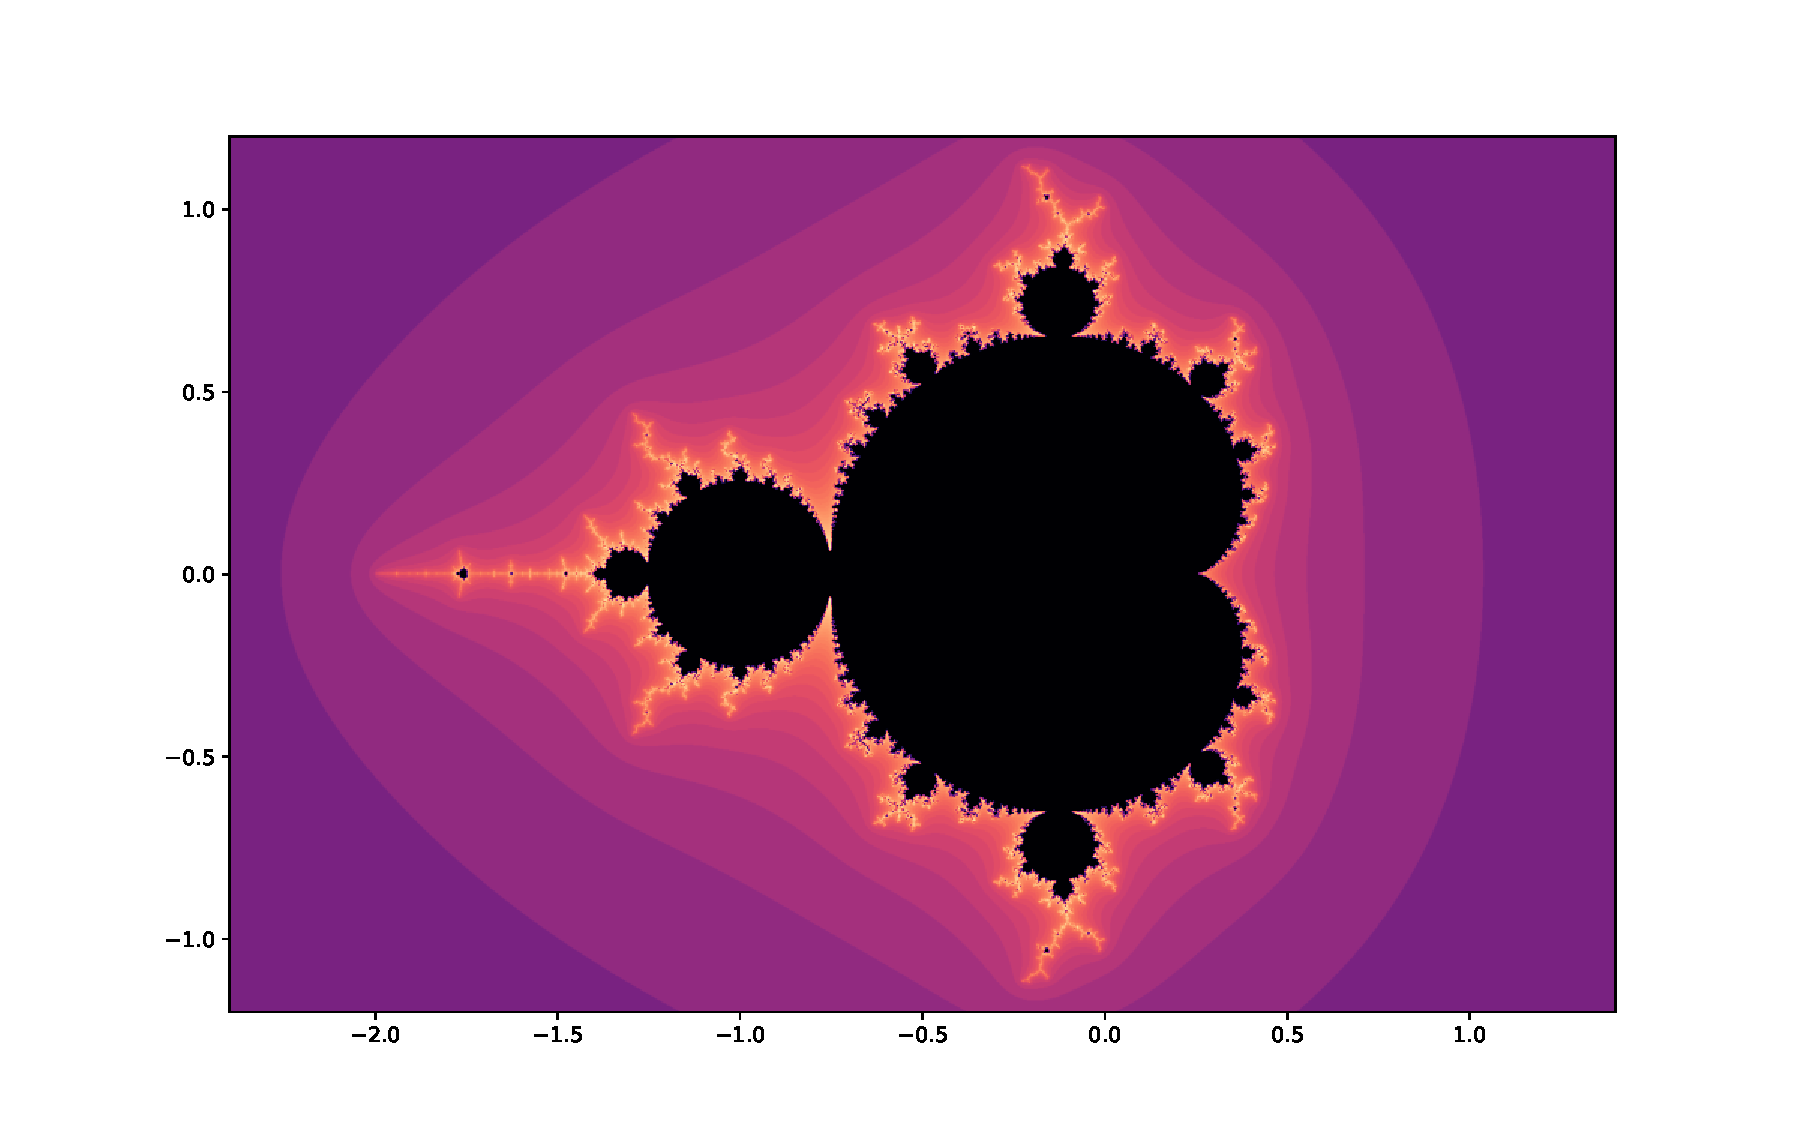
\includegraphics[width=\linewidth]{../Results/Figures/Mandelbrot.pdf}
    \caption{Mandelbrot set colored in black. The color of the other points is determined by the number of iterations needed to determine whether the sequence \eqref{eq:mandelbrot} diverges.}
    \label{fig:mandelbrot}
\end{figure}

\section*{Data Analysis}

The data analysis in this template covers a simple process of processing and plotting data. The growth of cell clusters is tracked at discrete times. Therefore, we are interested in the total number of cells over time as well as the actual increase of cell numbers for each time step. This is visualized in Figure \ref{fig:cell_growth}.

\begin{figure}
    \centering
    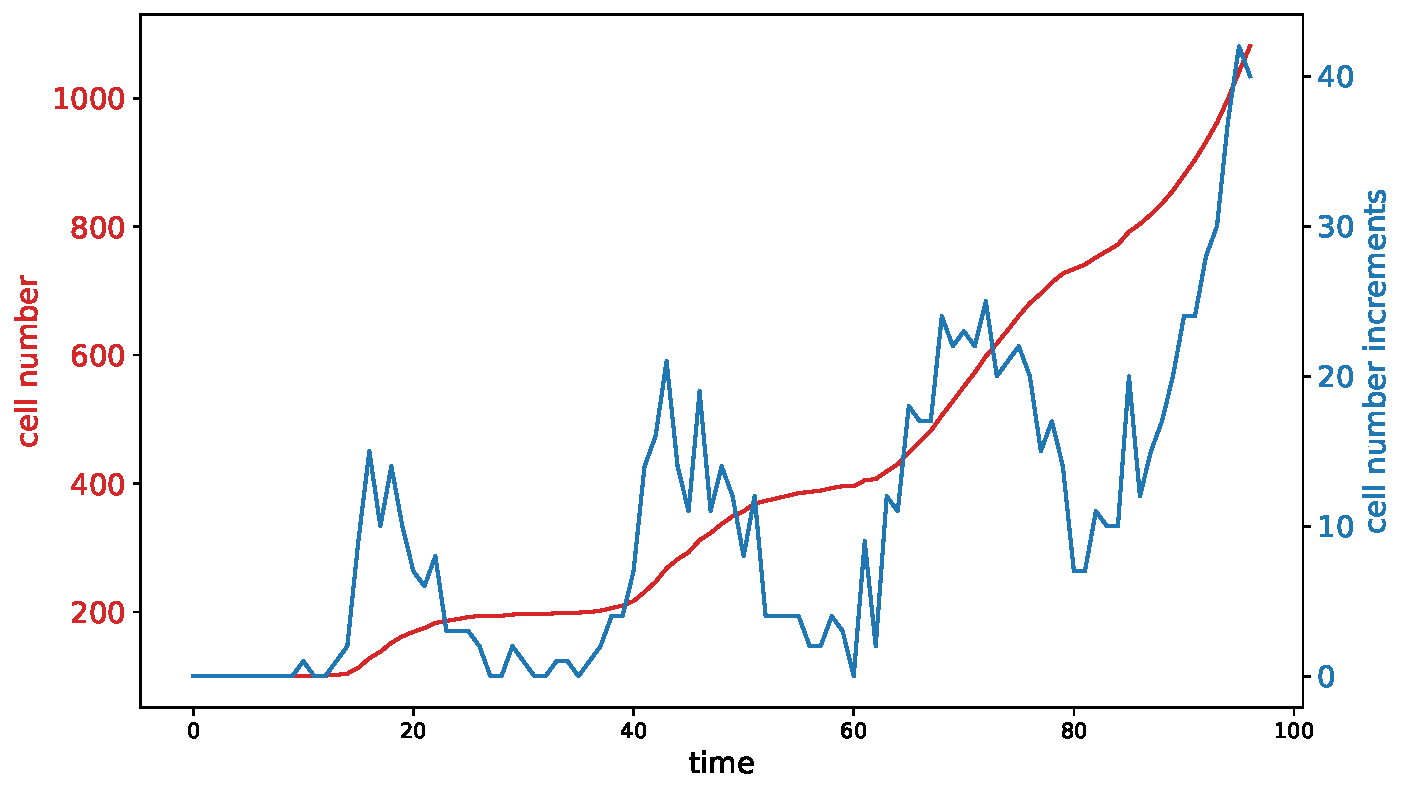
\includegraphics[width=\linewidth]{../Results/Figures/CellNumbers.pdf}
    \caption{Cell growth over time. The total number of cells is shown in blue, the increase of cells in orange.}
    \label{fig:cell_growth}
\end{figure}

Additionally it could be interesting to take a look at the spatial distribution of the cells themselves. This is shown in Figure \ref{fig:cell_distribution}.

\begin{figure}
    \begin{subfigure}{0.49\textwidth}
    \centering
    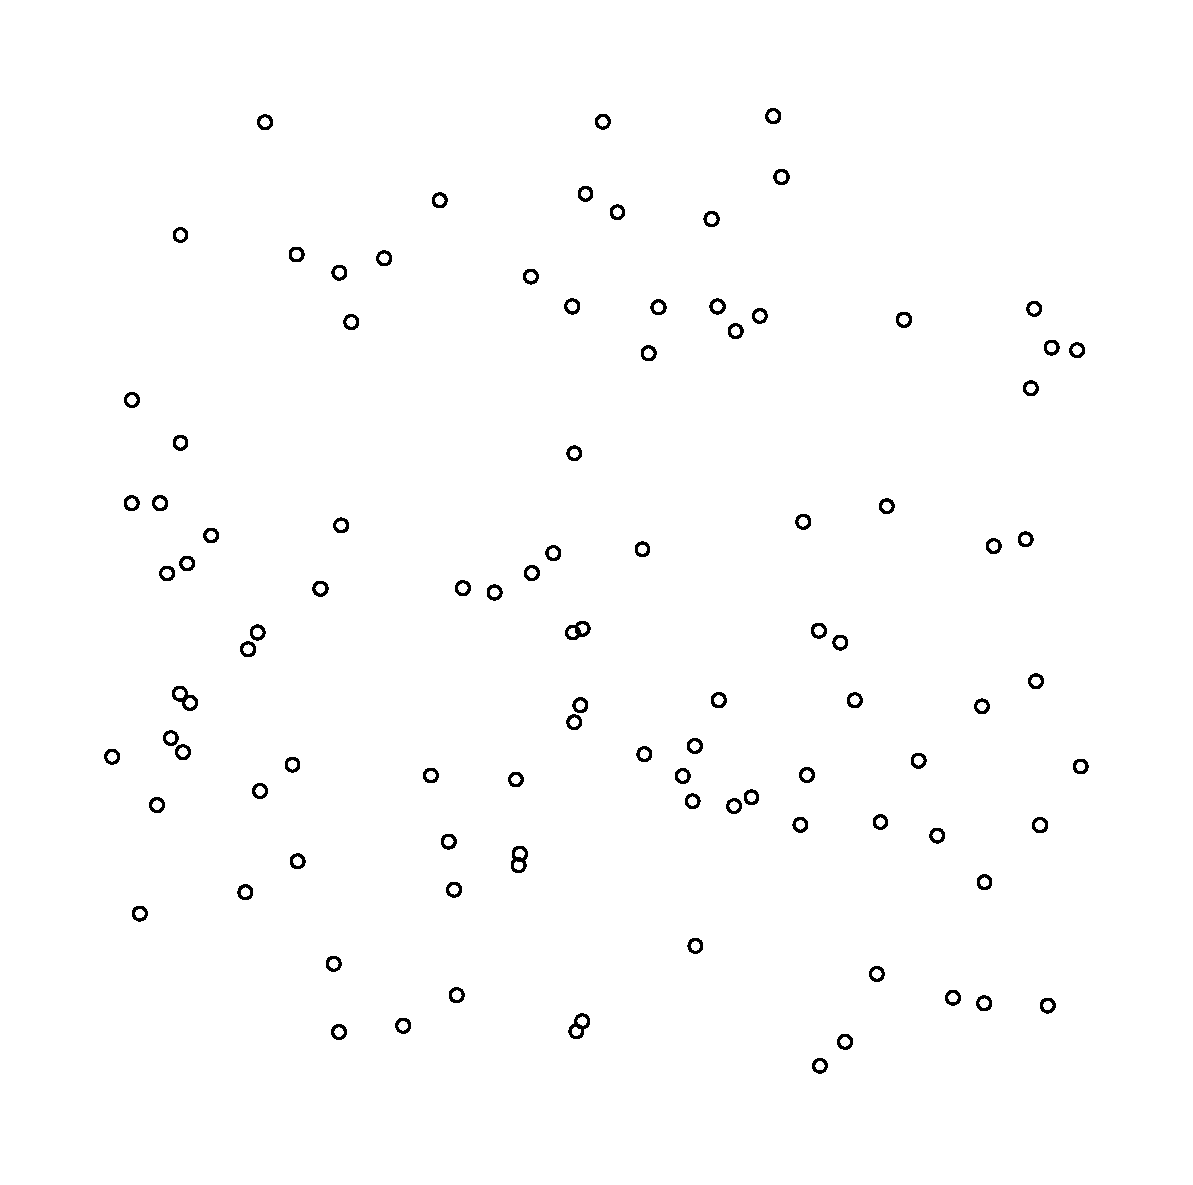
\includegraphics[width=\linewidth]{../Results/Figures/CellClusters_T=0.pdf}
    \subcaption{$T=0$}   
    \end{subfigure}
    \begin{subfigure}{0.49\textwidth}
        \centering
        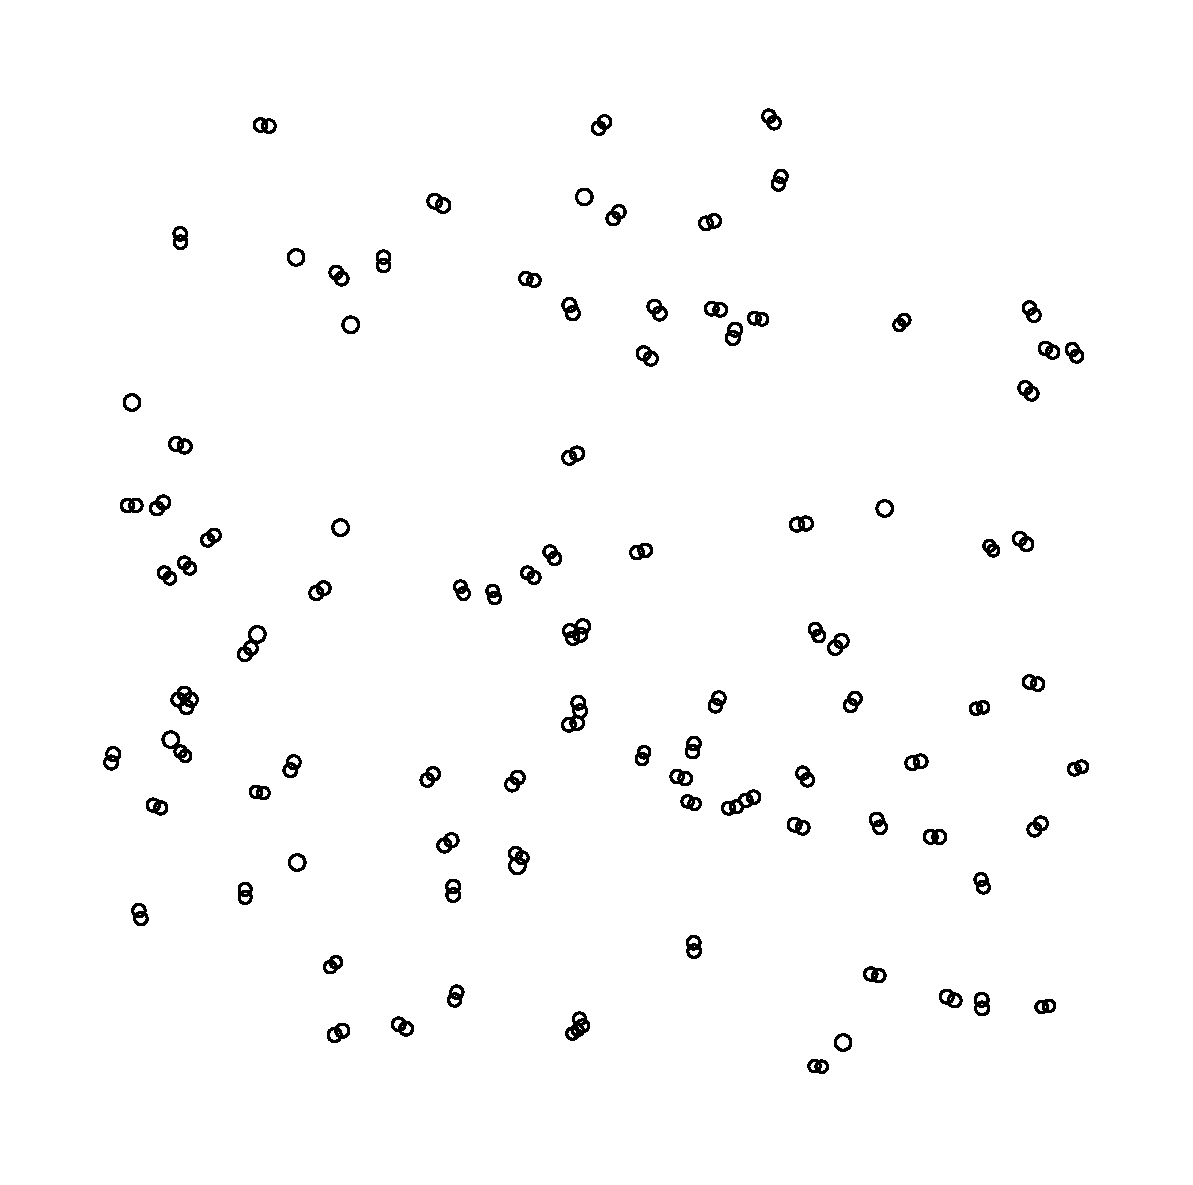
\includegraphics[width=\linewidth]{../Results/Figures/CellClusters_T=24.pdf}
        \subcaption{$T=24$}   
    \end{subfigure}
    \begin{subfigure}{0.49\textwidth}
        \centering
        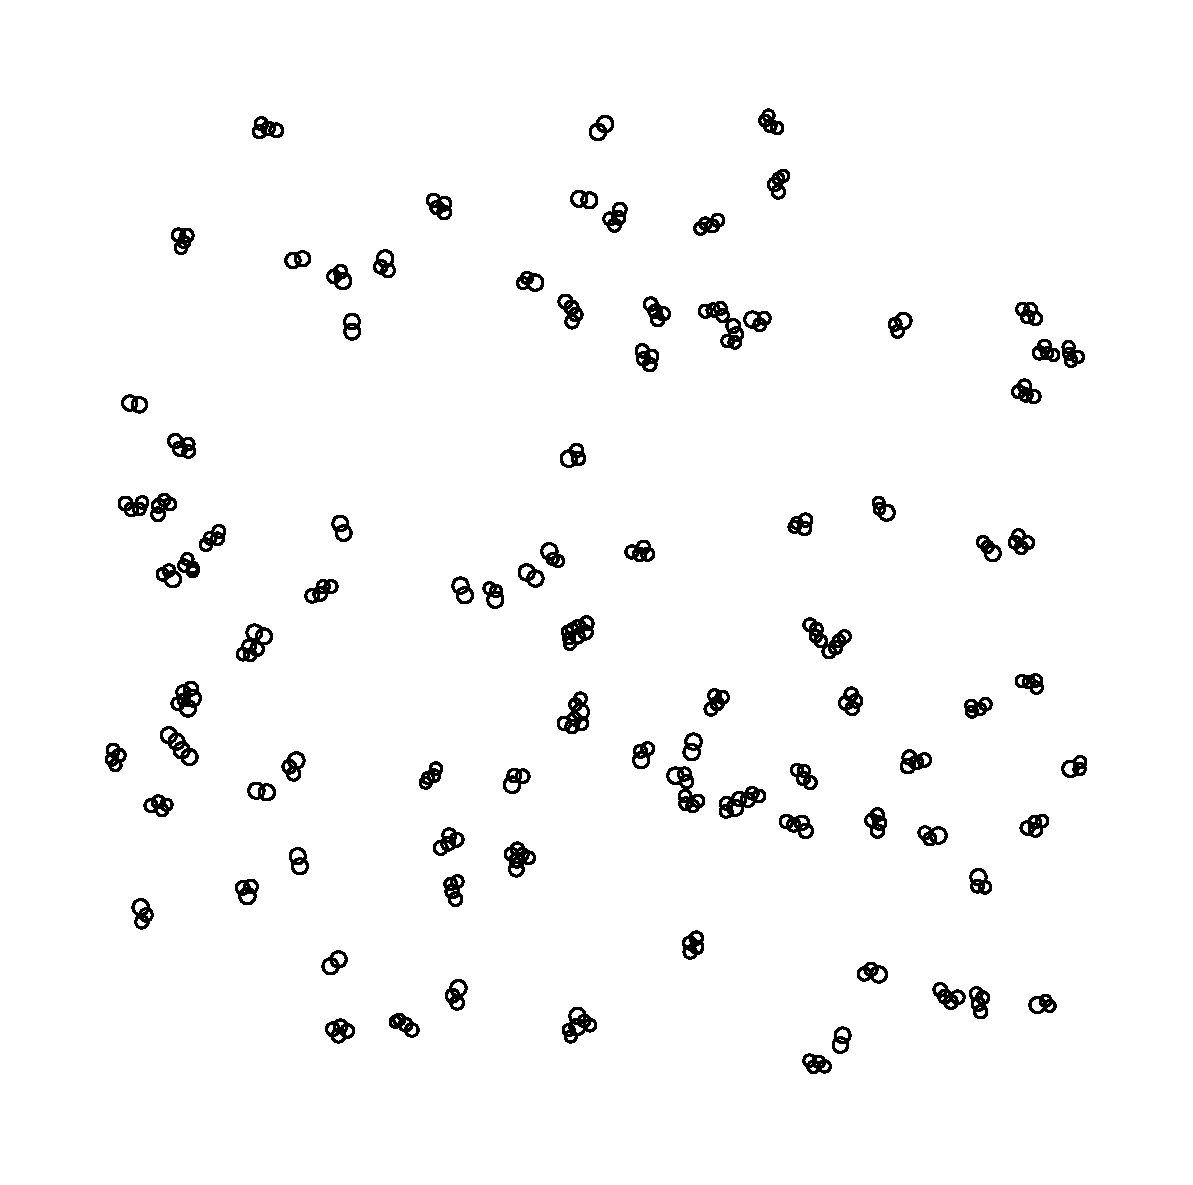
\includegraphics[width=\linewidth]{../Results/Figures/CellClusters_T=48.pdf}
        \subcaption{$T=48$}   
    \end{subfigure}
    \begin{subfigure}{0.49\textwidth}
        \centering
        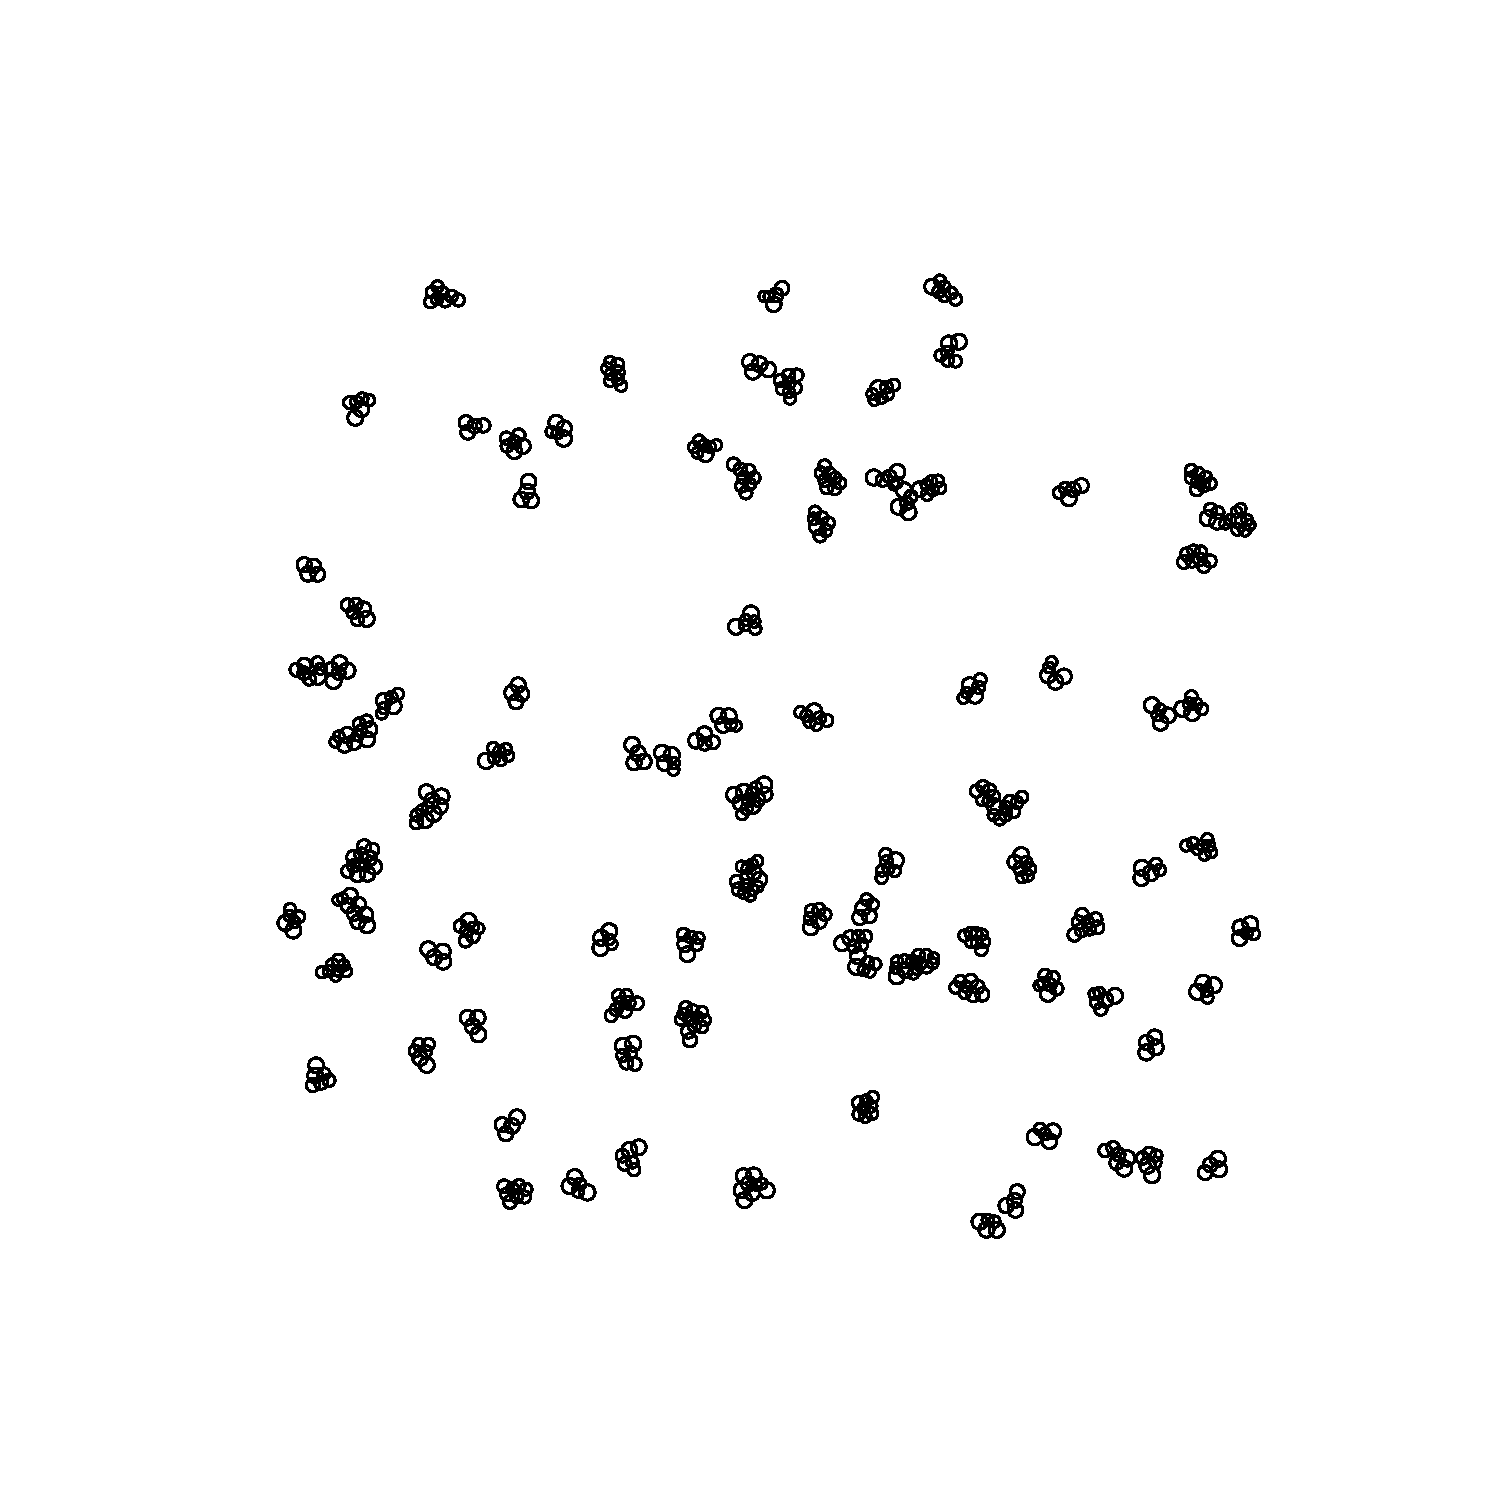
\includegraphics[width=\linewidth]{../Results/Figures/CellClusters_T=72.pdf}
        \subcaption{$T=72$}   
    \end{subfigure}
    \caption{Spatial distribution of the cells at different points in time.}
    \label{fig:cell_distribution}
\end{figure}

\section*{Additional Information}

In total, this template aims to give you a general picture of how your project might be structured. It is not meant to be a strict guideline since any project comes with its own individual quirks. Feel free to add or remove sections as you see fit. Always ask yourself the question whether a completely unrelated person could at least understand the general idea of your project by reading not only the manuscript but also the code and the documentation.

I would also like to mention some of the tools involved in the creation of this template, as they might be useful for you as well:
\begin{enumerate}
    \item Python programming was done in Visual Studio Code with the Python extension.
    \item The manuscript was written in Visual Studio Code usind the \LaTeX extension.
    \item Most of the comments and docstrings were generated using GitHub copilot.
    \item Version control is done using Git and GitHub.
\end{enumerate}
\textbf{With that being finished, have fun with your own project!}

\end{document}